%%%%%%%%%%%%%%%%%%%%%%%%%%%%%%%%%%%%%%%%%%%%%%%%%%%%%%%%%%%%%%%%%%%%%%%%
% Plantilla TFG/TFM
% Escuela Politécnica Superior de la Universidad de Alicante
% Realizado por: Jose Manuel Requena Plens
% Contacto: info@jmrplens.com / Telegram:@jmrplens
%%%%%%%%%%%%%%%%%%%%%%%%%%%%%%%%%%%%%%%%%%%%%%%%%%%%%%%%%%%%%%%%%%%%%%%%

\chapter{Results}\label{chap:results}

In this chapter we will go through the results obtained from the experiments
performed in the previous chapter. We will start by evaluating the predictive
performance of our model, followed by a discussion of the results and their
implications.

\section{Evaluation}

\begin{figure}
    \centering
    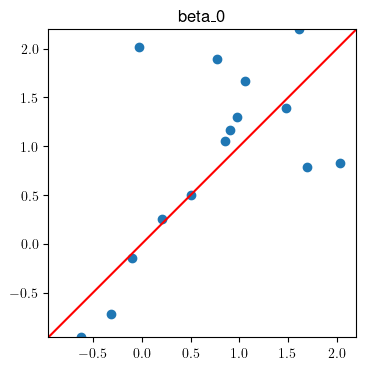
\includegraphics[width=0.3\textwidth]{files/plots/scatter/beta_0.png}
    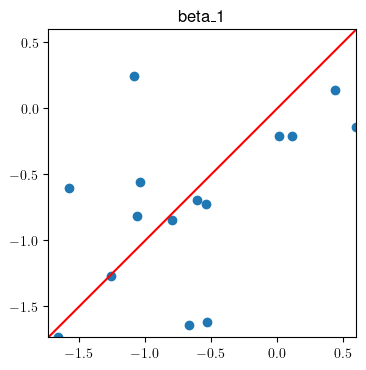
\includegraphics[width=0.3\textwidth]{files/plots/scatter/beta_1.png}
    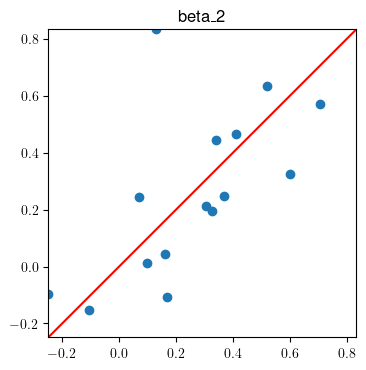
\includegraphics[width=0.3\textwidth]{files/plots/scatter/beta_2.png}
    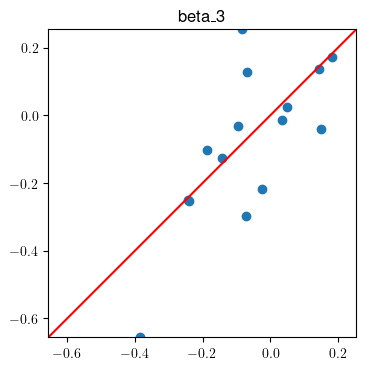
\includegraphics[width=0.3\textwidth]{files/plots/scatter/beta_3.png}
    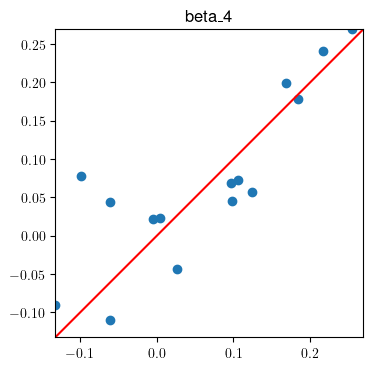
\includegraphics[width=0.3\textwidth]{files/plots/scatter/beta_4.png}
    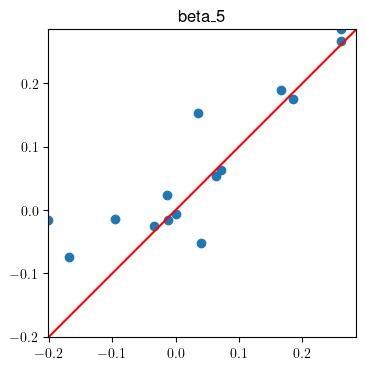
\includegraphics[width=0.3\textwidth]{files/plots/scatter/beta_5.png}
    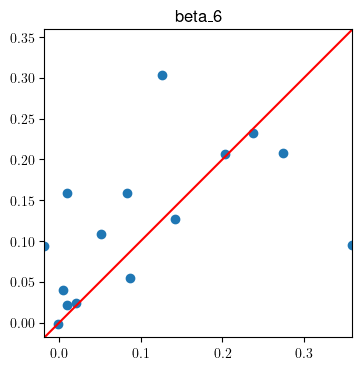
\includegraphics[width=0.3\textwidth]{files/plots/scatter/beta_6.png}
    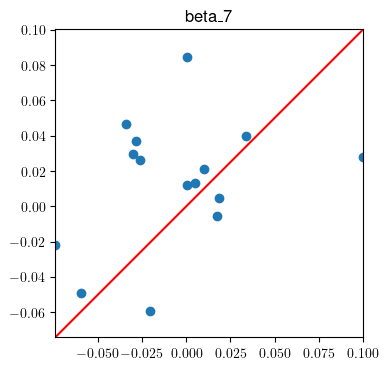
\includegraphics[width=0.3\textwidth]{files/plots/scatter/beta_7.png}
    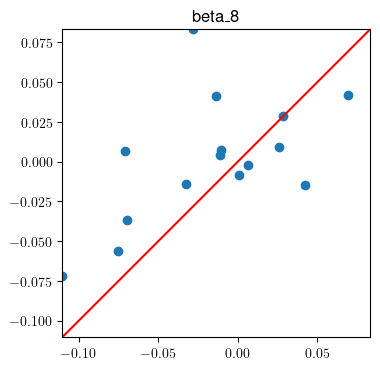
\includegraphics[width=0.3\textwidth]{files/plots/scatter/beta_8.png}
    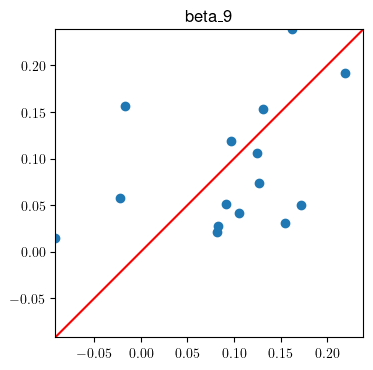
\includegraphics[width=0.3\textwidth]{files/plots/scatter/beta_9.png}
    \caption{Predictions vs ground truth}
    \label{fig:scatter}
\end{figure}

\subsection{Quantitative results}

The mean \gls{mae} of the model in the test set when predicting the $\beta$
parameter is \textbf{0.064}. Figure \ref{fig:scatter} shows the predictions of
the model vs the ground truth, and Table \ref{tab:mae} shows the \gls{mae} for
each $\beta$. We can see that the model is able to predict the correct value in
most cases, but it has some problems with outliers.

\begin{table}[h]
    \centering
    \caption{\gls{mae} for each $\beta$ parameter}
    \begin{tabular}{ c c }
        \toprule
        \textbf{Feature} & \textbf{MAE} \\
        \midrule
        $\beta_1$        & 0.107        \\
        $\beta_2$        & 0.129        \\
        $\beta_3$        & 0.076        \\
        $\beta_4$        & 0.065        \\
        $\beta_5$        & 0.017        \\
        $\beta_6$        & 0.027        \\
        $\beta_7$        & 0.025        \\
        $\beta_8$        & 0.021        \\
        $\beta_9$        & 0.041        \\
        $\beta_{10}$     & 0.025        \\
        \bottomrule
        \label{tab:mae}
    \end{tabular}
\end{table}

\subsection{Qualitative results}
\begin{figure}[h]
    \centering
    \begin{subfigure}{\textwidth}
        \centering
        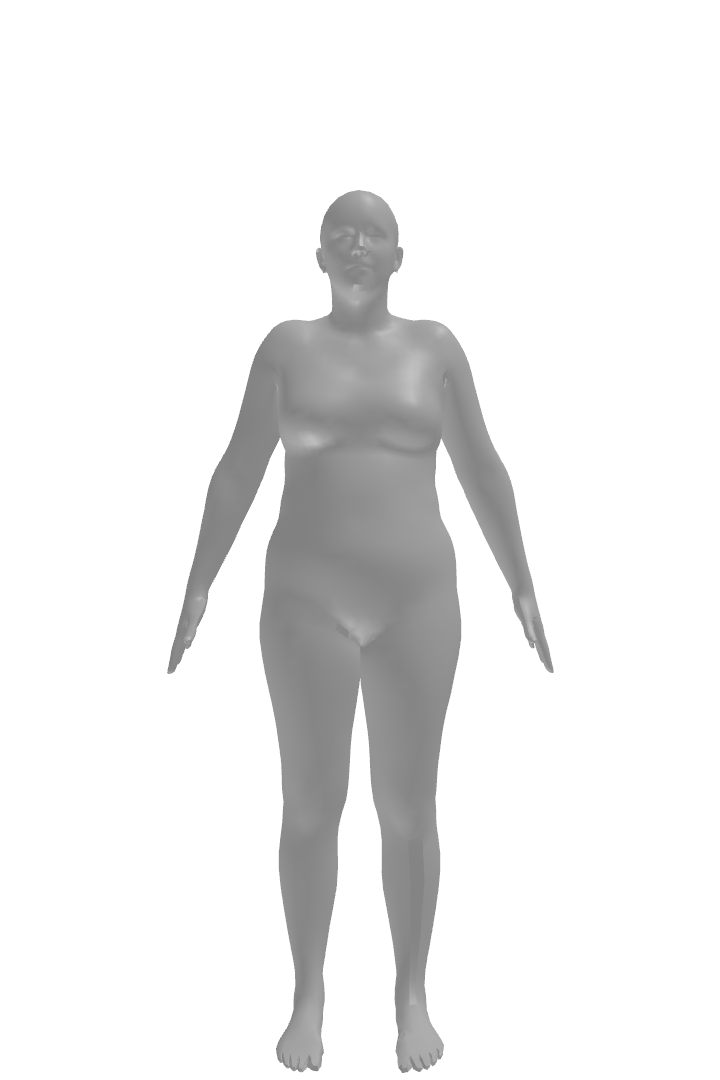
\includegraphics[width=60pt]{files/patients/9_2}
        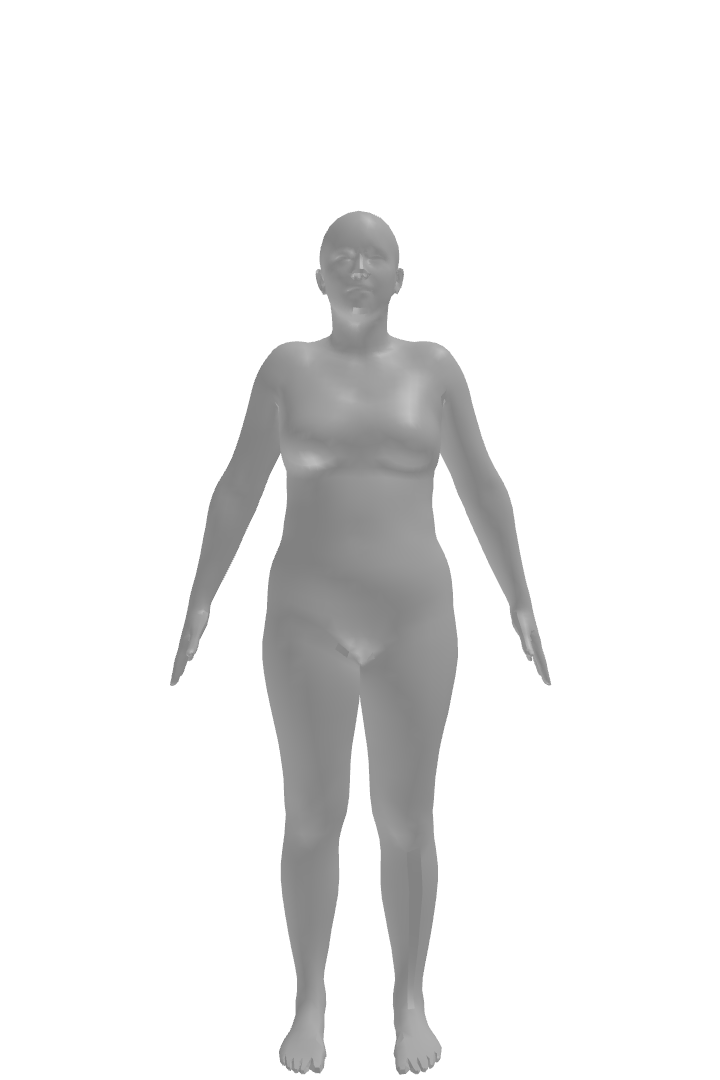
\includegraphics[width=60pt]{files/patients/9_3}
        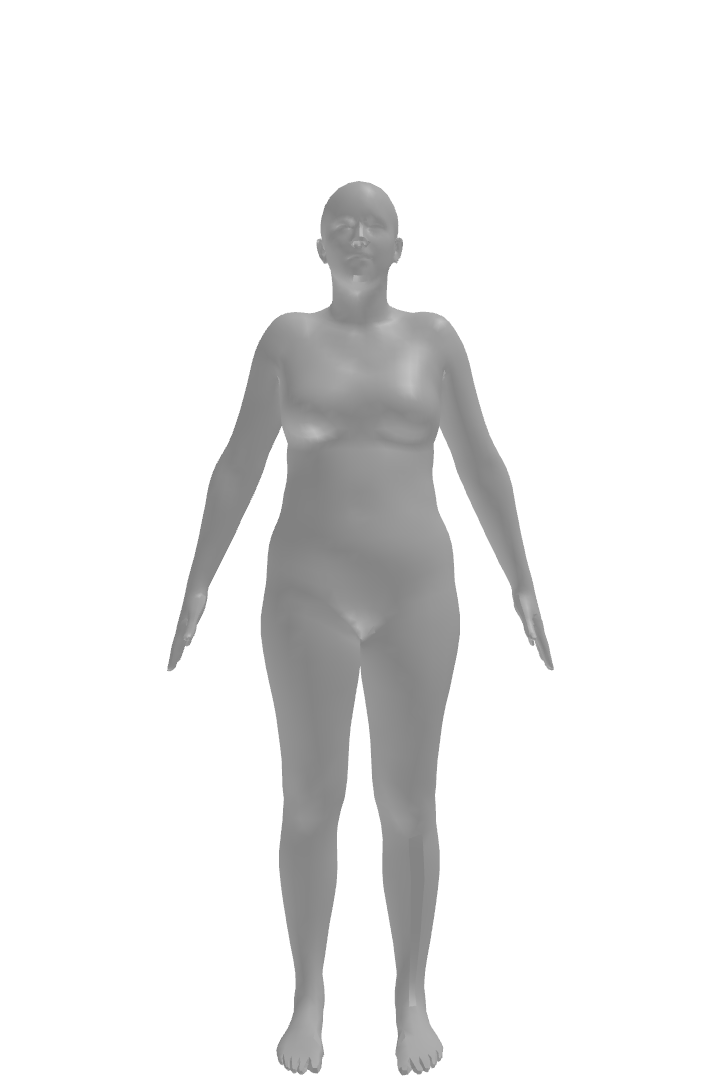
\includegraphics[width=60pt]{files/patients/9_4}
        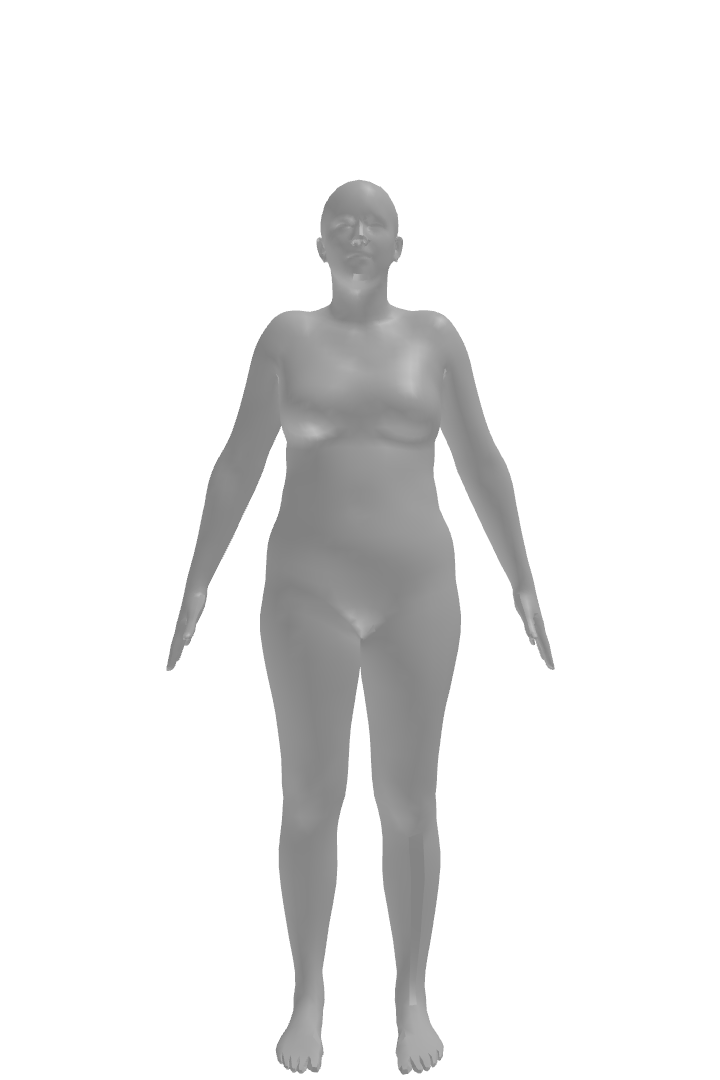
\includegraphics[width=60pt]{files/patients/9_5}
        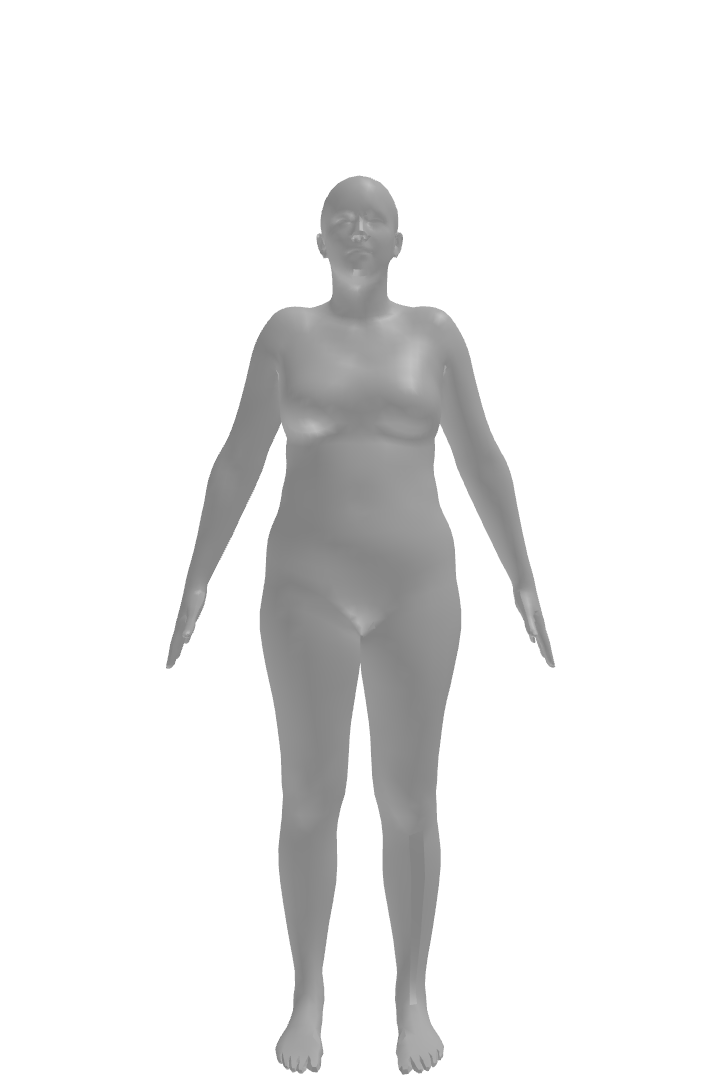
\includegraphics[width=60pt]{files/patients/9_6}
        \hspace{10pt}
        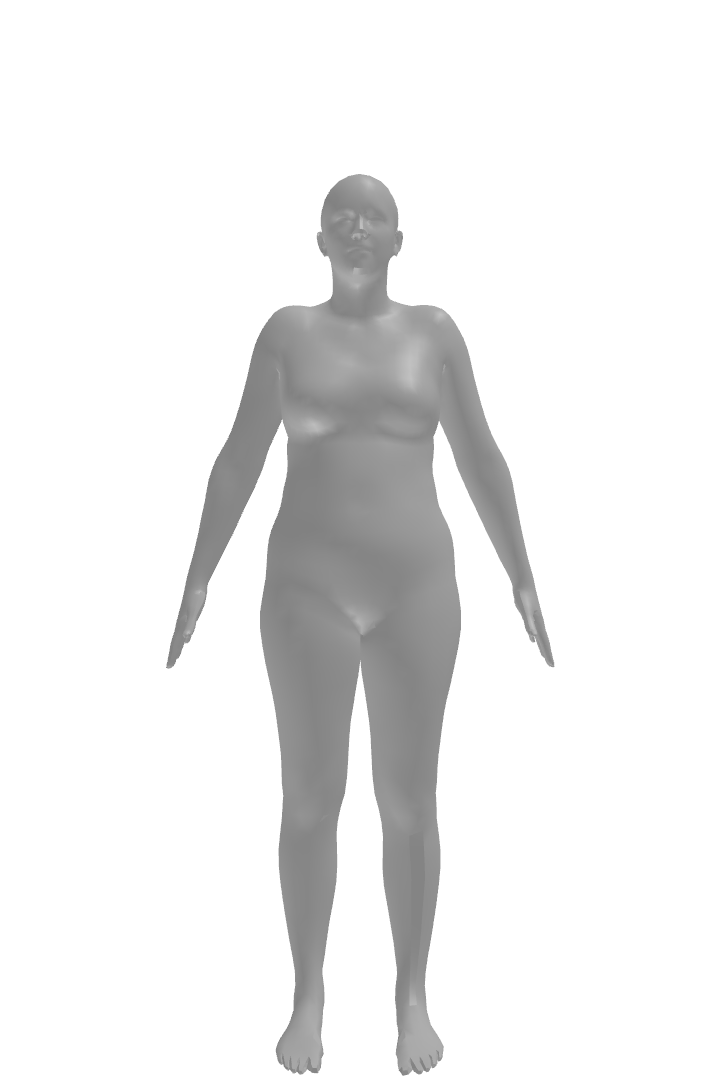
\includegraphics[width=60pt]{files/patients/9_predicted}
    \end{subfigure}
    \linebreak
    \begin{subfigure}{\textwidth}
        \centering
        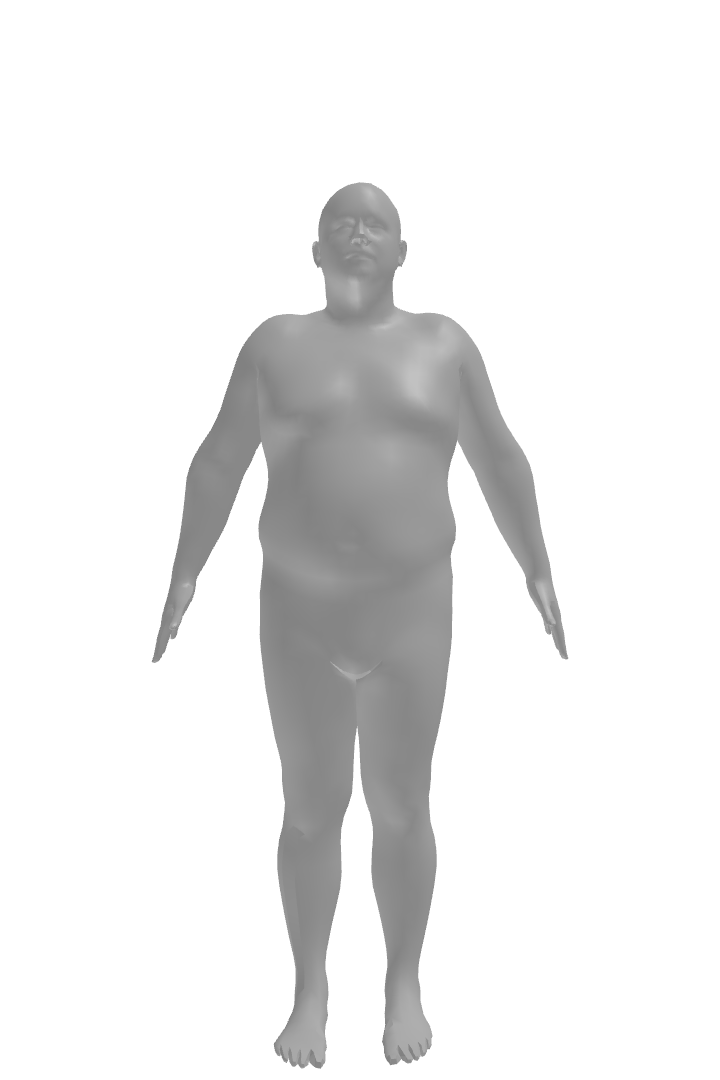
\includegraphics[width=60pt]{files/patients/128_1}
        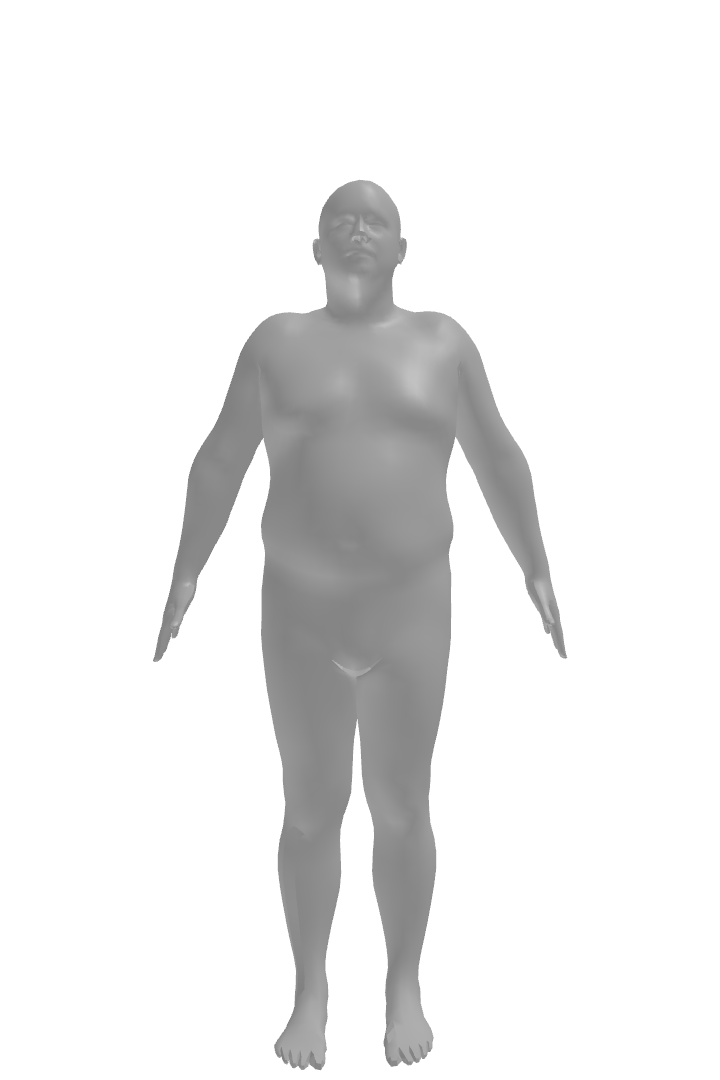
\includegraphics[width=60pt]{files/patients/128_2}
        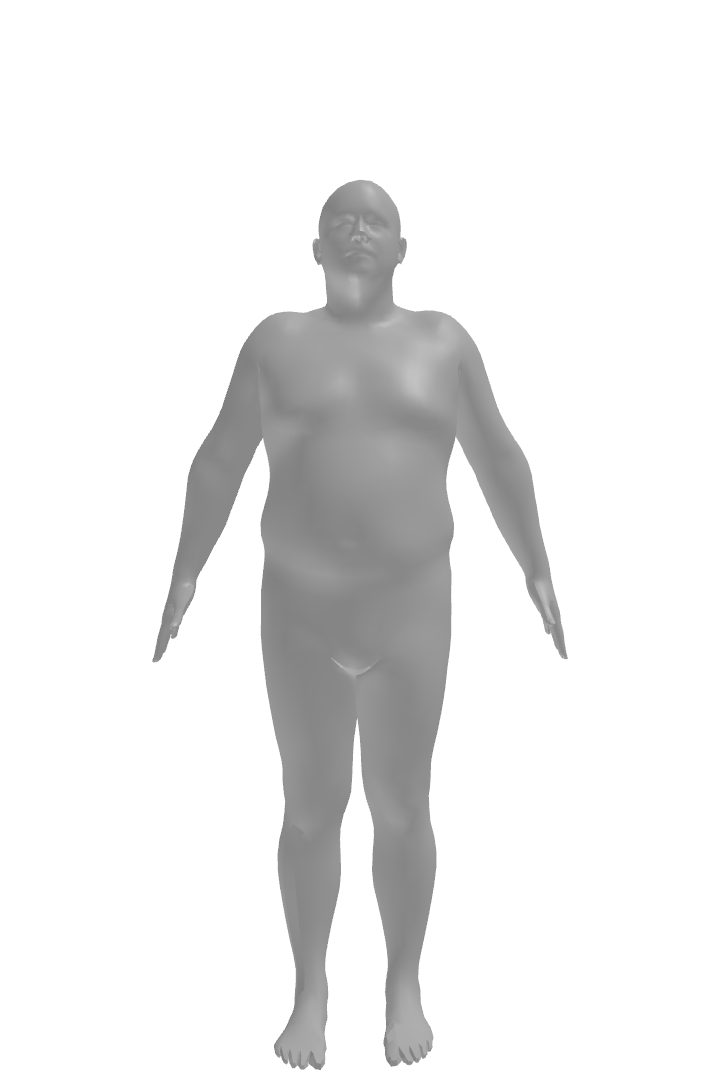
\includegraphics[width=60pt]{files/patients/128_3}
        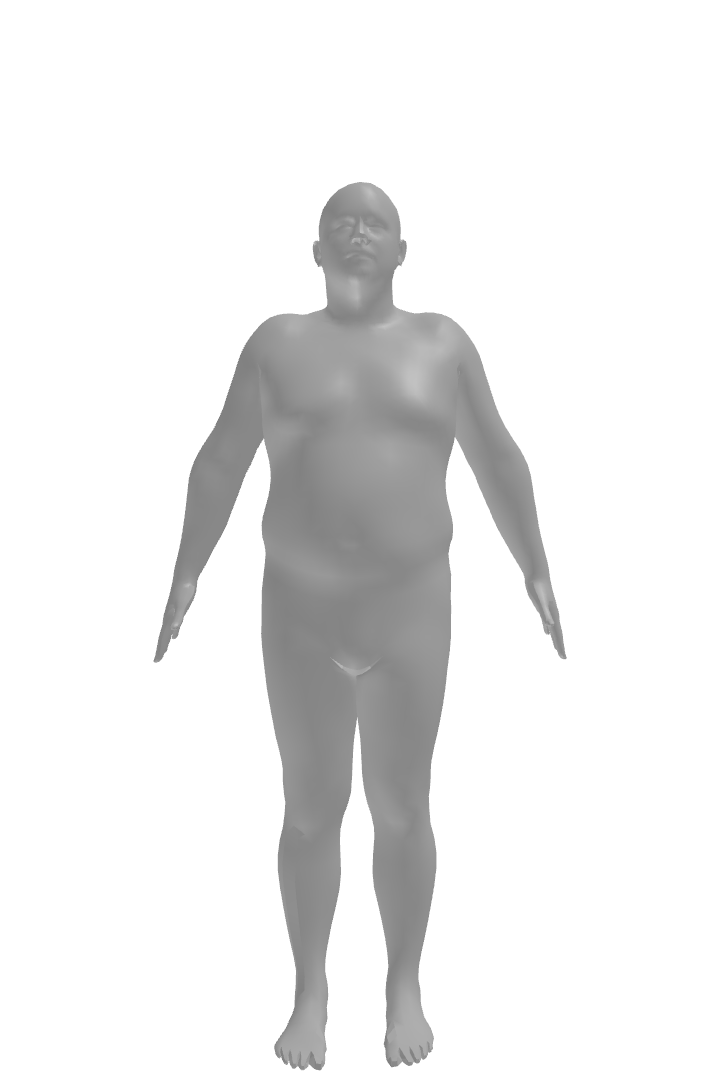
\includegraphics[width=60pt]{files/patients/128_4}
        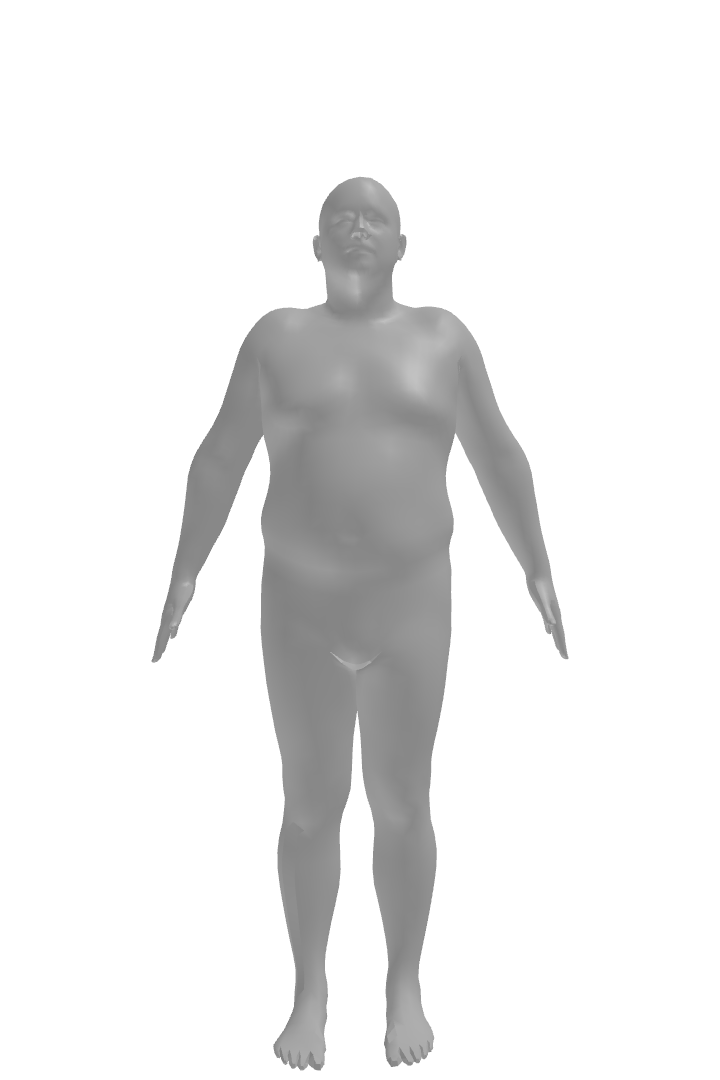
\includegraphics[width=60pt]{files/patients/128_5}
        \hspace{10pt}
        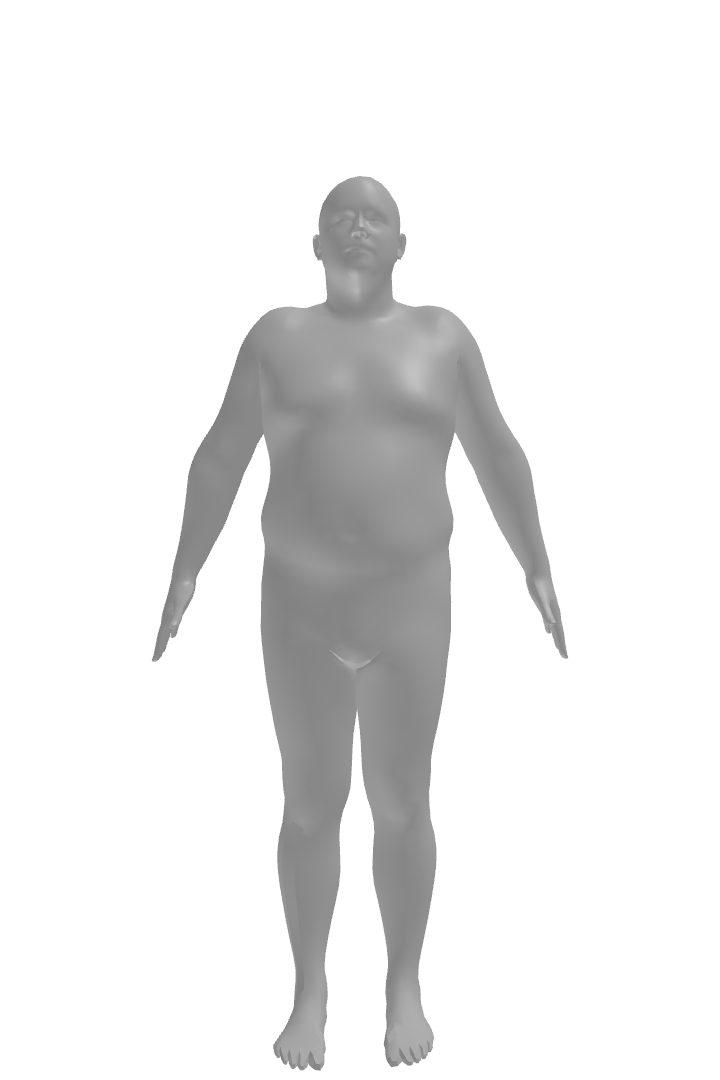
\includegraphics[width=60pt]{files/patients/128_predicted}
    \end{subfigure}
    \caption{Predicted bodies for two patients.}
\end{figure}

\section{Discussion}

\begin{figure}[h]
    \centering
    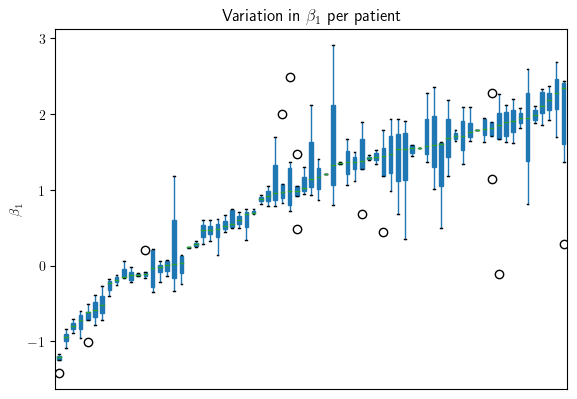
\includegraphics[width=\textwidth]{files/beta_1_var.png}
    \caption{Variation of $\beta_1$ in the dataset per patient.}
    \label{fig:beta-var}
\end{figure}

One of the main problems of the model is that it has a lot of variance in
$\beta_1$. This parameter controls the overall height of the person (Figure
\ref{fig:beta-1-vis}). This has the effect of making the generated human bodies
vary in height, which is not desirable.

This is probably due to the fact that the training data has a lot of variance
in height, which is probably due to scanning error or our method of extracting
the \gls{smpl} parameters from the scans. Figure \ref{fig:beta-var} shows the
variation of $\beta_1$ in the dataset per patient.

To mitigate this problem, several solutions can be explored. One potential
solution is the improvement of data preprocessing, specifically in the
extraction of the SMPL parameters from the scans. By refining this process, the
quality of the training data can be significantly enhanced, reducing the
variance in the $\beta_1$ parameter and leading to more accurate predictions.

Alternatively, we could consider incorporating a form of regularization into
our model specifically targeted at controlling the variation in the height
parameter. By including a penalty term in our loss function that encourages
consistency in the height parameter, we can influence the model to maintain
more stable height predictions across sequences.

Finally, it is also possible to investigate the use of post-processing
techniques. For instance, once the model makes a prediction, we can adjust the
$\beta_1$ value based on a running average from previous sessions, thus
ensuring more consistency in the predicted height.